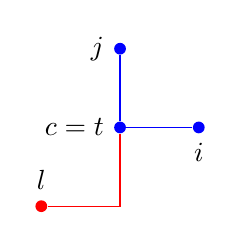
\begin{tikzpicture}

    % Blue points forming an L-shape
    \node[fill=blue, circle, inner sep=1.5pt, label=left:{\(\boldvec{c}=\boldvec{t}\)}] (c) at (0, 0) {};
    \node[fill=blue, circle, inner sep=1.5pt, label=below:{\(\boldvec{i}\)}] (i) at (1, 0) {};
    \node[fill=blue, circle, inner sep=1.5pt, label=left:\(\boldvec{j}\)] (j) at (0, 1) {};
    
    % Draw lines to form the L-shape
    \draw[blue] (c) -- (i);
    \draw[blue] (c) -- (j);
    
    % Red point near the L-shape
    \node[fill=red, circle, inner sep=1.5pt, label=above:\(\boldvec{l}\)] (l) at (-1, -1) {};
    
    % Connect the red point to the blue L-shape with another L-shape
    \draw[red] (l) -- (0,-1) -- (c) ;
    
\end{tikzpicture}